\begin{example}
	\index{Example: HMC Hamiltonian variable change}
	Let $\xi \equiv e^\zeta$, such that $\zeta\in [-\infty,\infty]$ maps to $\xi\in[0,\infty]$ and $\xi$ is ensured to be positive definite regardless of the value of $\zeta$. Using the differential $d\xi =  \xi d\zeta$ in \EQref{eq:q3} means $p(\theta,\xi,\lambda|D,I)$ is multiplied with $\xi$. Hence, when taking $-\ln(p(\theta,\xi,\lambda|D,I))$ according to \EQref{eqh}, a $-\ln(\xi)$ is added to the Hamiltonian. In practice this means
	\begin{equation}
		(1-\tilde{\alpha})\ln(\xi)\in H\Rightarrow -\tilde{\alpha}\ln(\xi).
	\end{equation} 	
\end{example}



\begin{example}
	Suppose there is a game between a Robot and Nature in which the Robot objective is to guess the position of the Robot. The Robot is given measurements of its velocity and acceleration, at any time step and must formulate a belief about its position. Nature decides the true position of the Robot and will penalize the Robot according to the deviation between the Robots estimate of its position and the true position viz (\dfref{def:quadratic_cost})
	\begin{equation}
		C(U(x),s) = (U(x)-s)^2,
	\end{equation}
	where $s$ is the true position $U(x)$ is the Robots estimate based on data $x$ containing velocity and acceleration measurements. 
	\begin{figure}[H]
		\centering
		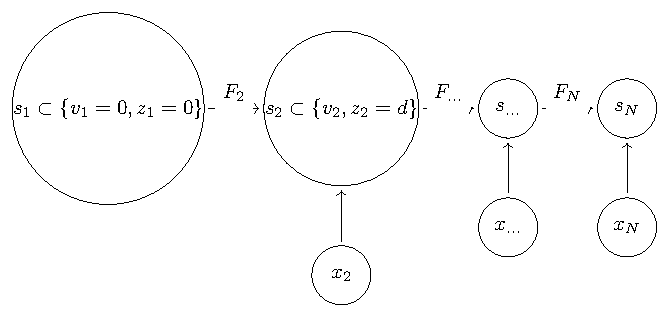
\includegraphics[width = 0.8\textwidth]{figures/graph.pdf}
		\caption{}
		\label{fig:1}
	\end{figure}
	Suppose the Robot is given all historical data, then the expected cost can be written
	\begin{equation}
		\mathbb{E}_{S|X}[C(U(X),S|s_1,\{x\}_{2:N},I)] = \int ds (U(x_N)-s)^2p(s|s_1,\{x\}_{2:N},I).
	\end{equation}
	The optimal decision is defined by
	\begin{equation}
		\frac{d}{dU(X)}\bigg(\mathbb{E}_{S|X}[C(U(X),S|s_1,\{x\}_{2:N},I)]\bigg)\bigg|_{U(x_N)=U^*(x_N)} = 0
	\end{equation}
	leading to (\thref{theorem:expectation_decision_rule})
	\begin{equation}
		U^*(x_N) = \mathbb{E}[S_{N}|s_1,\{x\}_{2:N},I].
		\label{eq:dr}
	\end{equation}
	The inutitive interpretation of \EQref{eq:dr} is that the optimal decision of the Robot is to estimate the position that it expects Nature to have chosen. Now
	\begin{equation}
		\mathbb{E}[S_{N}|s_1,\{x\}_{2:N},I] = \int ds_{N} s_N p(s_N|s_1,\{x\}_{2:N},I).
		\label{eq:a5}
	\end{equation}
	Assume that
	\begin{equation}
		\begin{split}
			p(s_i|s_{i-1},I) &= N(s_i|\mu_i = F_is_{i-1}+b_i,\Sigma_i = Q_i),\\
			p(x_i|s_{i},I) &= N(x_i|\mu_i = H_is_{i}+d_i,\Sigma_i = R_i)
		\end{split}
		\label{eq:a2}
	\end{equation}
	Hence, $p(s_N|s_1,\{x\}_{2:N},I)$ must be reformulated such that the above can be utilized. 
	Now
	\begin{equation}
		\begin{split}
			p(s_N|s_1,\{x\}_{2:N},I) &= \frac{p(x_{N}|s_N,s_1,\{x\}_{2:N-1},I)p(s_N|s_1,\{x\}_{2:N-1},I)}{p(x_{N}|s_1,\{x\}_{2:N-1},I)}\\
			&= \frac{p(x_{N}|s_N,I)p(s_N|s_1,\{x\}_{2:N-1},I)}{p(x_{N}|s_1,\{x\}_{2:N-1},I)}\\
		\end{split}
		\label{eq:a3}
	\end{equation}
	where
	\begin{equation}
		\begin{split}
			p(s_N|s_1,\{x\}_{2:N-1},I) &= \int ds_{N-1}p(s_N,s_{N-1}|s_1,\{x\}_{2:N-1},I)\\
			&= \int ds_{N-1}p(s_N|s_{N-1})p(s_{N-1}|s_1,\{x\}_{2:N-1},I)\\
			&=N(s_{N}|\mu_{N|N-1},\Sigma_{N|N-1})
		\end{split}
		\label{eq:a1}
	\end{equation}
	where 
	\begin{equation}
		\begin{split}
			\mu_{N|N-1} &= F_{N}\mu_{N-1}+b_N\\
			\Sigma_{N|N-1} &= F_{N}\Sigma_{N-1}F_{N}^T+Q_{N}\\
		\end{split}
	\end{equation}
	Using \EQref{eq:a1} and \EQref{eq:a2} in \EQref{eq:a3} then yields~\citep{murphy2023probabilistic}
	\begin{equation}
		p(s_N|s_1,\{x\}_{2:N},I) = N(s_N|\mu_{N},\Sigma_N)
		\label{eq:a4}
	\end{equation}
	where
	\begin{equation}
		\begin{split}
			\mu_{N} &= \mu_{N|N-1}+K_N(x_N-\hat{x}_N),\\
			\Sigma_{N} &= \Sigma_{N|N-1}-K_NS_NK_N^T,\\
			K_N & = \Sigma_{N|N-1}H_N^TS_N^{-1},\\
			\hat{x}_N&= H_N\mu_{N|N-1}+d_N,\\
			S_N & = H_N\Sigma_{N|N-1}H_N^T+R_N\\
		\end{split}
	\end{equation}
	Combining \EQref{eq:a4} with \EQref{eq:a5} then yields the optimal decision for the Robot
	\begin{equation}
		\mathbb{E}[S_{N}|s_1,\{x\}_{2:N},I] = \mu_{N}.
	\end{equation}
	
\end{example}

\begin{example}
	Consider a Robot moving in one dimension. Every time interval $\Delta t$, the Robot will sample a wheel counter and an accelerometer. The wheel counter will be incremented every distance $d$. The Robot is interested in knowing its position and velocity. Expand the position viz
	\begin{equation}
		z(t+\Delta t)=z(t)+\Delta t \frac{dz(t)}{dt}+\frac{1}{2}(\Delta t)^2\frac{d^2z(t)}{dt^2}+\mathcal{O}(\Delta t^3)
	\end{equation}
	which discretize to
	\begin{equation}
		z_k\simeq z_{k-1}+\Delta t v_{k-1}+\frac{1}{2}(\Delta t)^2a_{k-1},
	\end{equation}
	where $\Delta t = \text{const}$ and
	\begin{equation}
		\begin{split}
			v_k &\simeq v_{k-1}+\Delta t a_{k-1},\\
			a_k &\simeq a_{k-1},
		\end{split}
	\end{equation}
	This means
	\begin{equation}
		\begin{split}
			s_k &= \begin{pmatrix}
				z_k\\ v_{k} \\ a_k\\
			\end{pmatrix}\\
			& \simeq \underbrace{\begin{pmatrix}
					1 & \Delta t & \frac{1}{2}\Delta t^2  \\
					0 & 1 & \Delta t  \\
					0 & 0 & 1  \\
			\end{pmatrix}}_{=F_k}\begin{pmatrix}
				z_{k-1}\\ v_{k-1} \\ a_{k-1}\\
			\end{pmatrix}
		\end{split}
	\end{equation}
	where $b_k=\emptyset$ for simplicity. Now take
	\begin{equation}
		\begin{split}
			x_k &= \begin{pmatrix}
				c_k \\ a_k
			\end{pmatrix}\\
			&= \underbrace{\begin{pmatrix}
					d^{-1} & 0 & 0\\
					0 & 0 & 1 
			\end{pmatrix}}_{=H_k}\begin{pmatrix}
				z_{k-1}\\ v_{k-1} \\ a_{k-1}\\
			\end{pmatrix}+r_k
		\end{split}
	\end{equation}
	where $r_k \sim N(0,R_k)$ with 
	\begin{equation}
		R_k = \begin{pmatrix}
			\sigma_z^2 & \sigma_z\sigma_a\\
			\sigma_z\sigma_a & \sigma_a^2 \\
		\end{pmatrix},
	\end{equation}
	where $\sigma_z$ and $\sigma_a$ are estimated from observations. The process noise can be determined viz~\href{https://github.com/rlabbe/Kalman-and-Bayesian-Filters-in-Python/blob/master/07-Kalman-Filter-Math.ipynb}{Kalman link}
	\begin{equation}
		Q_k = \begin{pmatrix}
			\frac{\Delta t^4}{4} & \frac{\Delta t^3}{2} & \frac{\Delta t^2}{2}\\
			\frac{\Delta t^3}{2} & \Delta t^2 & \Delta t\\
			\frac{\Delta t^2}{2} & \Delta t & 1\\
		\end{pmatrix}\sigma^2,
	\end{equation}
	where $\sigma \sim \Delta a$.
\end{example}
